% ---- ETD Document Class and Useful Packages ---- %
\documentclass{ucetd}
\usepackage{subfigure,epsfig,amsfonts}
\usepackage{natbib}
\usepackage{amsmath}
\usepackage{amssymb}
\usepackage{amsthm}

%% abbreviations %%
\usepackage{enumitem}
\newlist{abbrv}{itemize}{1}
\setlist[abbrv,1]{label=,labelwidth=1in,align=parleft,itemsep=0.1\baselineskip,leftmargin=!}

%% figure floating %%
\usepackage{float}

%% caption formatting %%
\usepackage{caption}
\captionsetup[figure]{font=normal}

%% appendix package? %%
\usepackage{appendix}
\usepackage{chngcntr}
\usepackage{etoolbox}

\AtBeginEnvironment{subappendices}{%
\chapter*{Appendix}
\addcontentsline{toc}{chapter}{Appendices}
\counterwithin{figure}{section}
\counterwithin{table}{section}
}

%% shortcut commands %%
\usepackage{xspace}
\newcommand{\UP}{\textsuperscript{+}\xspace} % +
\newcommand{\UM}{\textsuperscript{--}\xspace} % -
\newcommand{\U}[1]{\textsuperscript{#1}\xspace} % superscript general
\newcommand{\aLP}{$\alpha$LP\xspace} % aLP
\newcommand{\aLPs}{$\alpha$LPs\xspace} % aLPs
\newcommand{\ab}{$\alpha_4 \beta_7$} % a4b7
\newcommand{\Rora}{Ror$\alpha$} % Rora
\newcommand{\RORa}{ROR$\alpha$} % RORa
\newcommand{\RORgt}{ROR$\gamma$t} % RORgt
\newcommand{\abT}{$\alpha\beta$T\xspace} % abT
\newcommand{\gdT}{$\gamma\delta$T\xspace} % gdT
\newcommand{\IFNg}{IFN$\gamma$\xspace} % IFNg
\newcommand{\CDte}{CD3$\varepsilon$} % CD3e
\newcommand{\Ragrg}{Rag\U{--/--} Il2rg\U{--/--}\xspace} %Rag-/-Il2rg-/-

%% Use these commands to set biographic information for the title page:
\title{Computational and Experimental Studies of Potassium Channel Pore Domain Folding}
\author{Kevin C. Song}
\department{Biophysical Sciences}
\divisiona{The Physical Sciences}
\divisionb{The Biological Sciences}
\degree{Doctor of Philosophy}
\date{August, 2018}

%% Use these commands to set a dedication and epigraph text
\dedication{To my family, Louesa, Byungho, Jeungen, and Kelly}
\epigraph{"It doesn't matter how beautiful your theory is, it doesn't matter how smart you are. If it doesn't agree with experiment, it's wrong" - Richard Feynman}


\begin{document}
%% Basic setup commands
% If you don't want a title page comment out the next line and uncomment the line after it:
\maketitle
%\omittitle

% These lines can be commented out to disable the copyright/dedication/epigraph pages
\makecopyright
\makededication
\makeepigraph


%% Make the various tables of contents
\tableofcontents
\listoffigures
\listoftables

\acknowledgments
First, I would like to thank my academic advisors Dr. Beno\^{i}t Roux and Dr. Tobin Sosnick for their guidance throughout my thesis project. The nature of my thesis project was highly explorative, and without their patience and excellent guidance, this project would not have been able to be completed and fluorish. I really appreciate them both for giving me the intellectual freedom to learn how to be creative and teach me how to be a good scientist. \par

I would also like to thank my thesis committee members Dr. Eduardo Perozo and Dr. Andrei Tokmakoff for their insightful suggestions and discussions regarding my project. Specifically, I would like to thank Eduardo for his help with my understanding of membrane protein biochemistry better and I would like to thank Andrei for helping me understand protein kinetics better. \par

I have been extremely blessed with helpful and talented lab members, and especially, Yiling Zhang, Jing Li, Younghoon Koh, Michael Baxa, Adam Zmyslowski, Josh Riback \par

The University of Chicago Biophysics program has been invaluable to me, providing financial support as well as many friendships that will last throughout life. Michele Wittels, Julie Feder and Adam Hammond have provided me with assistance and constant support to ease. Eugene Leypunskiy, Herman Gudjonson, Vaughn Spurrier, and Boleslaw Osinski provided me with invaluable support and friendships throughout my tenure at the University of Chicago. I would not have been able to finish the work without their support \par

Last but not least, I would like to thank my family members Louesa Song, Dr. Byung Ho Song, Jeungen Yu, Bruce Akin, Dr. Renea Akin and Kelly Song for their constant support throughout life and 


\abstract
\par
For many potassium channels, tetramerization domains in either N- or C-terminal of the pore domain are thought to assist in tetrameric assembly by increasing local concentrations of monomer subunits. However, the pore domain, containing two transmembrane and a re-entrant pore helix, by itself form tetramers. Here, we investigate how the structural dynamics of monomers and tetramerization domains affect tetramer assembly of the potassium channels. Using Molecular Dynamics (MD) simulations, Markov State Modeling (MSM), Nuclear Magnetic Resonance (NMR), and a gel-based refolding assay, we find that wild-type (WT) potassium channel monomers exist in a partially disordered state and this affects kinetics and thermodynamics of tetramerization. MSM for the monomer simulations show that ~80\% of the population having the two transmembrane helices separated. We introduce 2 cysteine mutations at the bottom of each of these helices to lock them in a native-like arrangement. A [1H, 15N]-TROSY-HSQC NMR spectrum of WT monomer in bicelles is poor due to aggregation and heterogeneity; however, the disulfide mutant shows a spectrum with well-dispersed peaks, suggesting that the disulfide mutant retains a native-like spectrum with limited heterogeneity on NMR time-scale. We perform a refolding study in liposomes and find that the kinetics is faster and the yield of tetramers is higher in the disulfide bonded native-like mutant. We suggest that WT monomers behave as partially disordered states in the bilayer with a high proclivity to misfold due to stable non-native helical tetramerization. The rate limiting step for the disulfide mutant is concentration independent suggesting that folding is limited by a unimolecular events such as insertion of the pore helix into a tetramer formed by the eight transmembrane helices. Refolding of full-length KcsA monomers is concentration dependent and addition of the tetramerization domain hinders the folding of disulfide mutant. We suggest that the tetramerization domain is for selectivity rather than stability of tetramers.

\mainmatter
% Main body of text follows

%% INTRODUCTION %%


%% BEGIN INTRODUCTION %%

\chapter{Introduction}
\section{Membrane Protein Folding}
Membrane proteins are the cell's gateway to its environment. Using a variety of membrane proteins, a cell transmits information, receives nutrients, shapes itself and responds to outside signals. Membrane proteins reside in lipid membranes, and they constitute more than 30\% of the entire proteome. Despite its functional importance and its abundance, our understanding of biochemical and biophysical properties of membrane proteins are still immature because of the difficulties working with membrane proteins experimentally. Membrane proteins easily aggregate because of its high hydrophobicity, and without the correct membrane mimetics, the protein structures can be easily disturbed.

Generally speaking, membrane proteins can be sub-divided into 2 classes (\textbf{Fig. \ref{fig:intro_f1}}): $\alpha$-helical and $\beta$-barrel membrane proteins. $\alpha$-helical membrane proteins are mainly found in the plasma membrane of eukaryotes, the inner membranes of bacterial cells, and sometimes in the outer membranes of bacteria. They constitute between 20 - 25\% of all open reading frames. On the other hand, $\beta$-barrel membrane proteins are mostly found in the outer membranes of bacteria, mitochondria and chloroplasts, and they constitute only a few percent of all open reading frames. The folding processes for $\alpha$-helical and $\beta$-barrel membrane proteins are very different comprising different sets of chaperones and mechanisms.

\begin{figure}[!ht]
\begin{center}
	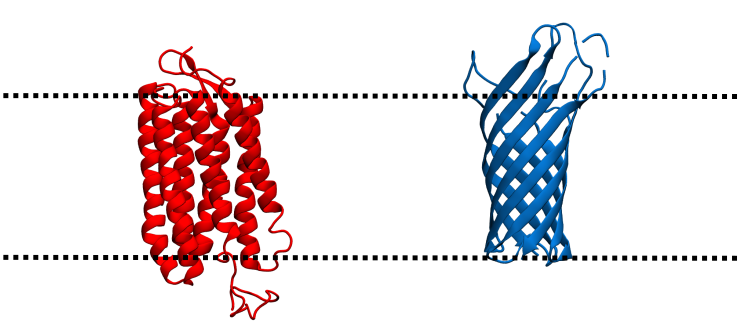
\includegraphics[width=\textwidth]{figures/introduction/Fig1/fig1.pdf}
\end{center}
	\caption{$\alpha$-helical versus $\beta$-barrel membrane protein}
Two representative structures of $\alpha$-helical and $\beta$-barrel membrane proteins are shown. Structure of bacteriorhodopsin (PDB ID: 1X0S) monomer is on the left in red, and OmpA (PDB ID: 1BXW) is shown on the right in blue. Hypothetical membrane boundaries are drawn in dashed black lines
	\label{fig:intro_f1}
\end{figure}

Individual $\alpha$-helices can be stable in the membrane as long as sidechains are hydrophobic enough; however, $\beta$-strands are not stable in the membrane because of exposed unsatisfied hydrogen donors and acceptors from the peptide backbone. Due to this difference in secondary structure, $\beta$-barrel membrane proteins insert and fold concurrently whereas $\alpha$-helical membrane proteins will insert one helix at a time and the helices rearrange to fold within the bilayer. In addition, $\beta$-barrel membrane proteins have been shown to fold reversibly from solution containing traditional denaturants such as urea and guanadine hydrochloride (GdnHCl) into lipids. (Fleming, Radford, Tamm, Rockwell) Because $\beta$-barrel membrane proteins can be monomeric and soluble in traditional denaturants, several proteins' (e.g. OmpA, OmpLA, OmpW, PagP) folding thermodynamics have been measured. In which, they found that they fold cooperatively by forming $\beta$ sheets at the lipid-water interface and insert. On the other hand, $\alpha$-helical membrane proteins are highly resistant to urea and GdnHCl, largely due to its hydrophobicity, and the denaturant of choice is sodium dodecyl sulfate (SDS) for folding studies of $\alpha$-helical membrane protein. With SDS, unfolded state of $\alpha$-helical membrane proteins still retain majority of its helicity. Because of this chemical property, most $\alpha$-helical membrane protein folding studies have focused on measuring folding thermodynamics and kinetics from SDS-unfolded states. 

The difference in folding mechanism is also reflected in how chaperones help these two classes of proteins fold. For $\beta$-barrel membrane proteins, BAM complexes have been shown to help them insert and fold by thinning the lipid bilayer thickness hence lowering the energy barrier to insert and fold. On the other hand, for $\alpha$-helical membrane proteins, ribosomes dock onto the SEC translocons and single helices are synthesized and inserted into the membrane one at a time as shown in \textbf{Figure \ref{fig:intro_f2}}. Many advances have been made in the field of $\beta$-barrel membrane proteins and there are excellent reviews available. (Fleming, Rockwell, Radford) Here in this thesis, the focus will be on the folding of $\alpha$-helical membrane proteins.

\begin{figure}[!ht]
\begin{center}
	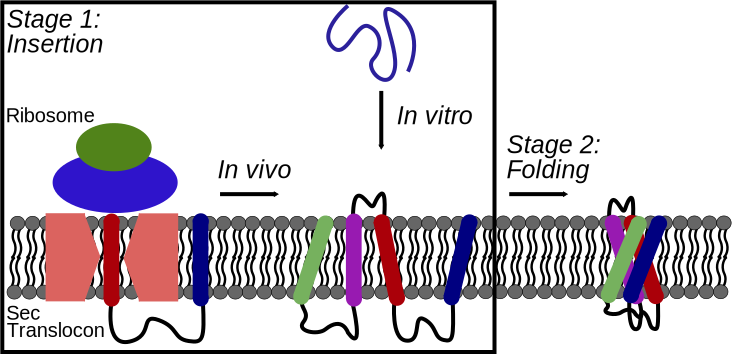
\includegraphics[width=\textwidth]{figures/introduction/Fig2/two_stage.pdf}
\end{center}
	\caption{Two-stage folding process for membrane protein folding.}
The first stage of the membrane protein folding process is insertion, where single helices are synthesized and inserted into the bilayer one at a time. As noted above, the insertion process is different for \textit{in vivo} and \textit{in vitro}. However, upon insertion of helices into the membrane, folding within the membrane is thought to process via the same pathway. 
	\label{fig:intro_f2}
\end{figure}

$\alpha$-helical membrane protein folding process is generally divided into 2 distinct stages (\textbf{Fig. \ref{fig:intro_f2}}). The first stage of membrane protein folding is called insertion, where the protein gets inserted into the membrane with native-like secondary structures. The exact mechanism on how a single helix transfers from inside the SEC translocon into the bilayer is not well understood yet, but the transfer is thought to happen via a lateral gate that opens in the translocon. Regardless, the insertion process is largely determined by the hydrophobicity of the peptide segment. Using amino acid hydrophobicity scales and sliding window averages, transmembrane segments can be well predicted. Yet, the prediction of final overall topology is still a difficult task. For some systems like LacY, the overall topologies can be flipped by changing the lipid compositions \textit{in vivo} and \textit{in vitro}.

After successful insertion of helices into the membrane, the helices begin to undergo a rearrangement process, which is described as folding within the membrane. This process is determined by many different forces including protein-protein and protein-lipid interactions. The major driving force for helix-helix interactions are not clear. Polar sidechain burial was thought of as a driving force for helix-helix associations; however, it was found



\section{Potassium Channels}
Potassium channels are found in all kingdoms of life. From bacteria to humans, potassium channels regulate the flow of K+ ions across cell membranes. In prokaryotes, these channels are responsible for cell growth and survival. In addition, biofilm, which is a community of bacterial cells, the microorganisms use potassium channels to communicate with each other. In higher order organisms like humans, potassium channels are used to drive muscle contraction and neuronal signaling.

The first structure of potassium channel was solved in 1998 by Roderick MacKinnon's lab, which he was awarded the Nobel Prize in Chemistry for in 2003. The structure showed that the pore is formed by juxtaposition of 4 subunits along the symmetry axis. The pore is lined with oxygen atoms from the backbone of the selectivity filter residues. Thes oxygen atoms provide binding sites for K+ ions as they pass through the pore. 


\section{Potassium Channel Folding}

%%\newpage
%%The aims of my studies are:
%%\begin{itemize}
%%\item Determine the structural state of potassium channel monomers in lipid bilayers
%%\item Determine the folding pathway of potassium channels
%%\end{itemize}

%% END INTRODUCTION %%



% Format a LaTeX bibliography
\makebibliography

% Figures and tables, if you decide to leave them to the end
%\input{figure}
%\input{table}

\end{document}


